\chapter{Návrh generátoru animace}

\section{Návrhový model}

Vzhledem k~tomu, že tento program je určen pouze pro zpracování vstupu na~náš výstup a~neexistují žádné trvalé mezistavy, není vůbec použita databáze a~s tím spojený databázový model.

\begin{figure}[h]
\centering
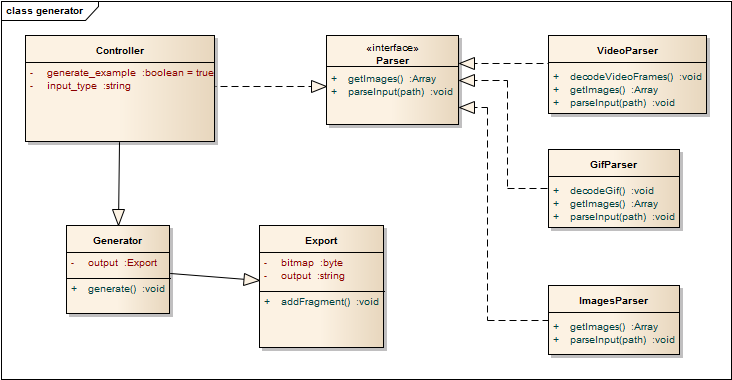
\includegraphics[width=1\textwidth]{figures/generator.png}
\caption{Návrhový model generátoru}
\label{fig:generator}
\end{figure}

\section{Popis tříd}

Následuje zde popis tříd generátoru animace. 

\subsection{Controller}
Controller je hlavní třída celého programu, která načítá všechny další služby pro správný běh programu. Stará se o~také o~kontrolu vstupu.

\subsection{Parser}
\label{secition:generatorparserclass}

Třídy, které implementují rozhraní Parser slouží k~načtení a~zpracování vstupu. Třída Controller načte vždy jen potřebný parser a~předá mu parametry pro načtení. Tato třída (resp. definovaná podtřída) převede vstup do unifikovaného formátu, který pak používá následující třída Generator. 

\subsection{Generator}

Tato třída obsahuje vlastní algoritmus pro vygenerování animace do našeho formátu, který je popsaný v~předchozí kapitole. Komunikuje s~výstupní třídou Exporter, kterému posílá výstupy.

\subsection{Exporter}

Třída Exporter se stará o~výstup aplikace. Vzhledem k~většímu počtu operací pro optimalizaci výstupu, zejména výstupu rastru velkého obrázku, je třeba tuto třídu definovat, nejedná se totiž pouze o~jednoduchý zápis do souboru. Stará se především o~minimalizaci výsledného formátu a~přidává přehrávací knihovnu.
